%\begin{figure}[!htpb]
%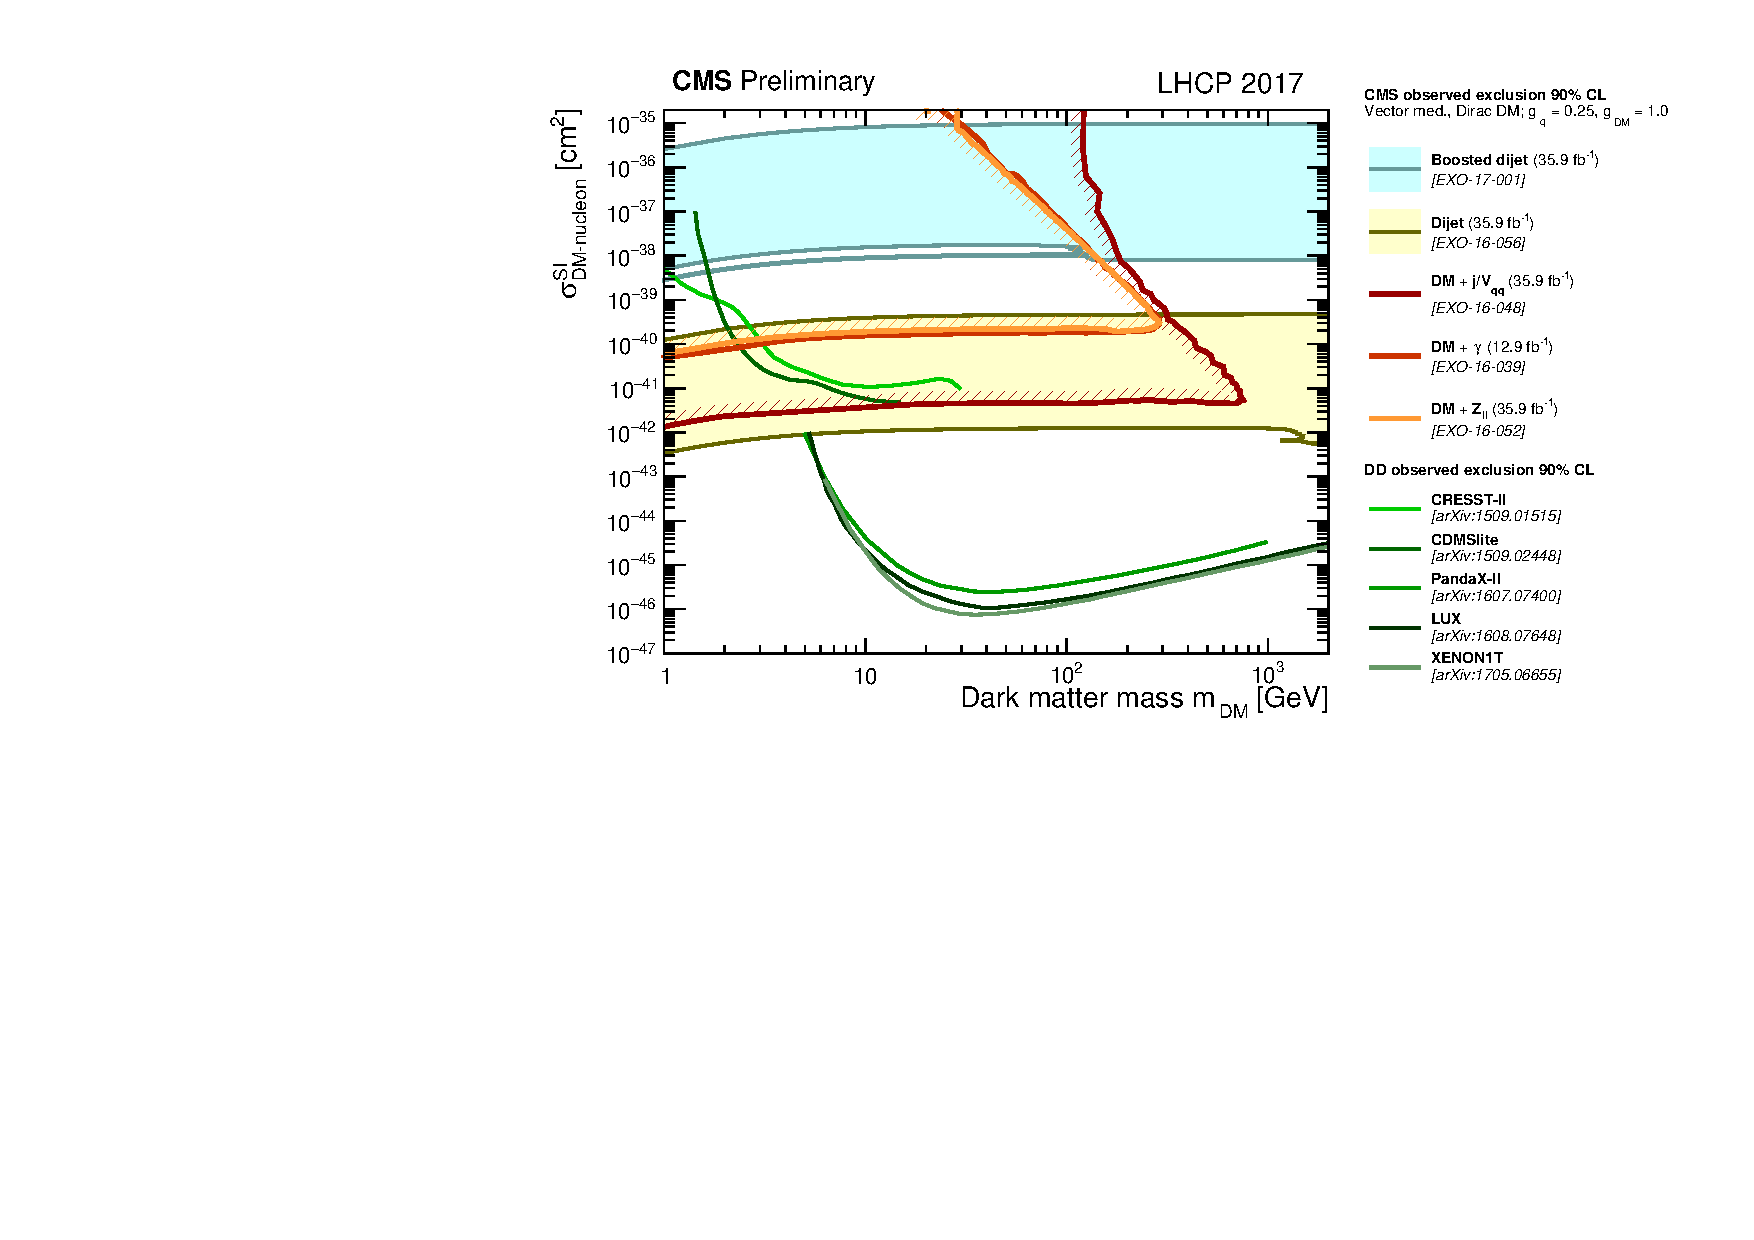
\includegraphics[width=0.9\textwidth]{figures/SI_CMSDD_Summary}
%\caption{
The 90\%-CL constraints from the CMS experiment 
from References \cite{Sirunyan:2017nvi,Sirunyan:2018xlo,Sirunyan:2017jix,CMS-PAS-EXO-16-053,Sirunyan:2017qfc}
in the \mdm-spin-independent DM--nucleon plane for a vector mediator,
Dirac DM, and benchmark couplings \gq = 0.25 and \gdm = 1.0 (marked as $g_{DM}$ in this plot) chosen as an example of what
early LHC searches would be sensitive to, compared with direct detection
experiments from References \cite{Angloher:2015ewa,Agnese:2015nto,Cui:2017nnn,Akerib:2016vxi,Aprile:2018dbl}. 
It is important to note that this comparison is only valid for this particular
combination of model and parameter choices. 
Abbreviation:\ DM, dark matter. Adapted from Reference~\citen{CMSSummary}.
%} 
%\label{fig:SICMS}
%\end{figure}